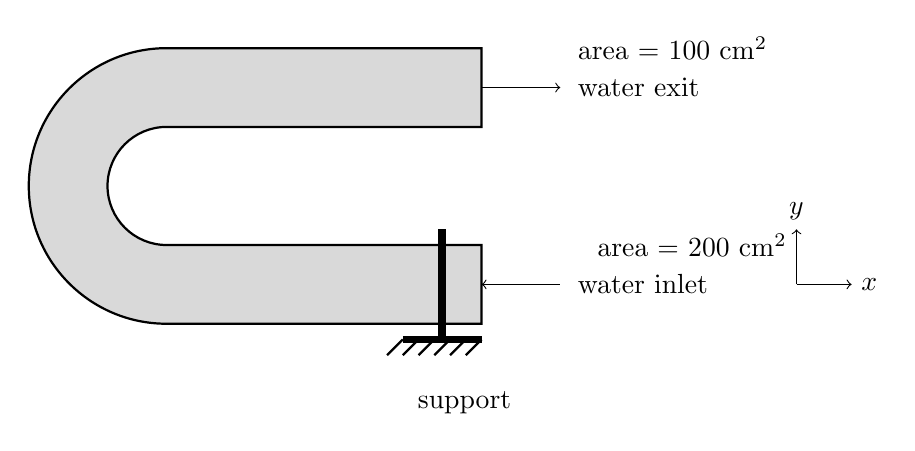
\begin{tikzpicture}
    \draw[thick, fill=gray!30] (0,0.5) -- (4,0.5) -- (4,1.5) -- (0,1.5) arc[start angle=270, end angle=90, radius=0.75] -- (0,3) -- (4,3) -- (4,4) -- (0,4) arc[start angle=90, end angle=270, radius=1.75]--(0,0.5) -- cycle;
    \draw[<-] (4,1) -- (5,1);
    \draw[->] (4,3.5) -- (5,3.5); 
    \node at (4.5,-0.5) [left] {support};
    \draw[line width=1mm](3.5,0.3)--(3.5,1.7);
    \draw[line width=1mm](3,0.3)--(4,0.3);
    \draw[thick](3,0.3)--(2.8,0.1);
    \draw[thick](3.2,0.3)--(3,0.1);
    \draw[thick](3.4,0.3)--(3.2,0.1);
    \draw[thick](3.6,0.3)--(3.4,0.1);
    \draw[thick](3.8,0.3)--(3.6,0.1);
    \draw[thick](4,0.3)--(3.8,0.1);
    \node at (7,1) [left] {water inlet};
    \node at (8,1.5) [left] {area = 200 cm$^2$};
    \node at (5.1,3.5) [right] {water exit};
    \node at (5.1,4) [right] {area = 100 cm$^2$};
    \draw[->] (8,1) -- ++(0.7,0) node[right] {$x$};
    \draw[->] (8,1) -- ++(0,0.7) node[above] {$y$};
\end{tikzpicture}

